

%method 



\setcitestyle{numbers,open={[},close={]}}
The lack of flexibility and accuracy of the core hole approximation combined with the computational deterrent of solving the BSE presents a barrier to expanding EELS calculations.  Lithium in particular, being highly sensitive to these effects requires an improved method to continue EELS studies.  To address this, a means of calculating the core hole shielding effect in lithium is developed.  It is based in the single particle approach so as to reduce computational effort and does not require any empirical results.  In this chapter the formulation and implementation of this method is discussed as well as the calculation and experimental parameters used in this work. 


\section{Improvement to Core Hole Shielding Calculations}
To improve ELNES simulations, the core hole shielding contribution must be calculated.   To maintain a low computational cost, the method developed here is based on a single particle approach.  In particular, the relativistic cross section method using the final state rule (FSR, Eq. \ref{telnes_eq}) \cite{jorissen2007ab}:

\begin{equation}
	\frac{\partial^2 \sigma}{\partial \Omega \partial E} = \left[\frac{4\gamma^2}{a_{\mathrm{0}^2q^4}}\right] \frac{k_f}{k_i} \sum_{i,f}|\mel{f}{e^{i\textbf{q}\cdot\textbf{r}}}{i}|^2\delta(E-E_f+E_i)
\end{equation}

As mentioned in Section \ref{Core Hole Approximation}, shielding effects are contained in the $\bra{f}$ term. These effects originate from changes in the Hamiltonian arising from the introduction of a core hole and manifest themselves when solving for $\bra{f}$ in the Kohn Sham equations (Eq. \ref{ks_eq}) \cite{kohn_self-consistent_1965}:  

\begin{equation}
    \bigg[T_i + V_{\mathrm{ext}}(\textbf{r}) + V_{\mathrm{H}}(\textbf{r}) + V_{\mathrm{XC}}(\textbf{r})\bigg] \phi_i(\textbf{r}) = \epsilon_i \phi_i(\textbf{r})
\end{equation}

The core hole alters the Hartree and the exchange and correlation potentials, and this effect is reduced somewhat by shielding.  The total change in the potential due to introduction of a core hole can be expressed as: 
\begin{equation}
\Delta V_{\mathrm{tot}}(\textbf{r})=\Delta V_{\mathrm{H}}(\textbf{r}) +\Delta V_{\mathrm{XC}}(\textbf{r})=V_{\mathrm{CH}}(\textbf{r}) - V_{\mathrm{S}}(\textbf{r})
\label{delta_potentials}
\end{equation}

where $V_{\mathrm{CH}}(\textbf{r})$ is the potential of a core hole and  $V_{\mathrm{S}}(\textbf{r})$ represents the shielding potential.  The current convention in literature when performing core hole calculations is to ignore this shielding term, despite the large effects it has been shown to have on ELNES.  The shielding potential can be divided into two parts, core electron shielding $V_{\mathrm{c}}(\textbf{r})$ and valence electron shielding  $V_{\mathrm{v}}(\textbf{r})$. Core shielding is due to electrons occupying core orbitals on the excited atom reducing how much the core hole can be ``felt" outside of the atom.  Valence screening is caused by valence and interstitial electrons being attracted to the positively charged hole.  Neither of these terms are readily solvable for using current methods.  When calculating ELNES for the lithium K edge, the core electron screening can be ignored.  This assumption arises from lithium's low electron count and simplifies the screening calculation considerably. \\

The valence electron screening can be calculated through linear response theory, as  $\Delta V_{\mathrm{H}}(\textbf{r})$ and $\Delta V_{\mathrm{XC}}(\textbf{r})$ cannot be computed exactly  \cite{shirley_modeling_2005}.  Linear response theory relates changes in electron density to changes in potential, such as from the introduction of a core hole, as described by Shirley, Soininen and Rehr is \cite{shirley_modeling_2005}:

\begin{equation}
\Delta n(\textbf{r}) = \int d^3 \textbf{r'} \chi^0(\textbf{r},\textbf{r'}; \omega = 0)\Delta V_{\mathrm{tot}}(\textbf{r'})
\end{equation}

Where $\chi^0$ is the irreducible polarization function, given by $\chi^0(\textbf{r}) = \delta n(\textbf{r}) /  \delta V(\textbf{r})$.  At this point, the screening is set to zero ($V_{\mathrm{S}}(\textbf{r})=0$), to be reintroduced later as a perturbation.  Restricting the region of interest to only the excited atom gives:
\begin{equation}
\Delta n _{\mathrm{basin}} = \int_{f}d^3\textbf{r} n_{f}(\textbf{r}) - \int_{i}d^3\textbf{r} n_i(\textbf{r})= -1
\label{density_calc}
\end{equation}
Where the basin defining the integration limits is defined by Bader theory as described in Section \ref{bader-theory}. This equation indicates that, when there is no screening,  the excited core electron has entirely left the basin, with no response from the material. Assuming that the polarization is constant inside this basin, lets the polarization to be calculated as: 

\begin{equation}
\frac{\Delta n _{\mathrm{basin}}}{V_{\mathrm{CH}}} = \chi^0_{\mathrm{basin}} = \frac{\Delta n _{\mathrm{basin}}}{\Delta V_{\mathrm{tot}}}
\label{chi_naught}
\end{equation}

The polarization further assumed as constant through changes in shielding potential, verified by checking that $\Delta n _{\mathrm{basin}}$ vs $V_{\mathrm{CH}}$ is linear, see Fig \ref{linearity}. The shielding term can then be reintroduced by perturbing the right hand side of Eq. \ref{chi_naught} to obtain: 


\begin{equation}
\frac{-1}{V_{\mathrm{CH}}} = \frac{-1+\delta n_{\mathrm{basin}}}{V_{\mathrm{CH}}-\delta V_{\mathrm{v}}}
\label{pertubation}
\end{equation}
Which can be reduced to:
\begin{equation}
\frac{\delta V_{\mathrm{v}}}{V_{\mathrm{CH}}} = \delta n_{\mathrm{basin}}
\label{final_eq}
\end{equation}

Equation \ref{final_eq} connects the screening due to valence electrons to a change in electron density, a rapidly calculable quantity.  The screening potential is given in ``units" of the core hole potential which allows the screening to be accounted for by modulating the occupancy of the core hole state.  Additionally, while perturbed from the no screening case in Eq. \ref{pertubation}, it should be noted that this argument holds when approached from the full screening case.  This indicates that these approximations are valid over the entire range of screening cases ($\delta V_{\mathrm{v}} = 0 \to V_{\mathrm{CH}}$).  The implementation of this theory in EELS calculations is discussed below.  

\begin{figure}
	\centering
	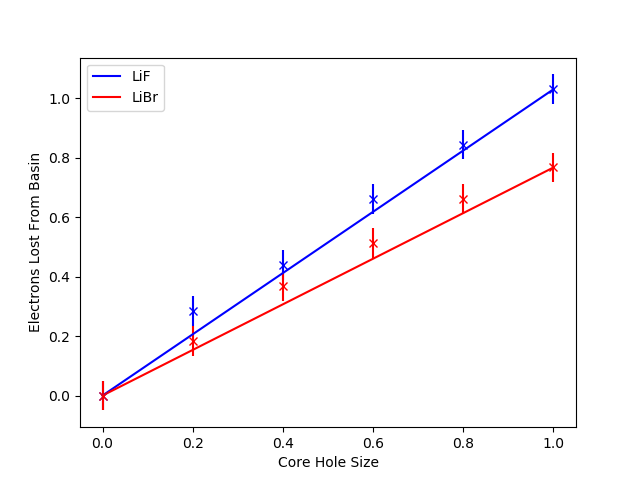
\includegraphics[width=0.55\textwidth]{linearity.png}
	\caption{Effect  of varying the core hole potential on atomic basin population, for LiF and LiBr.  Solid lines represent the case of constant $\chi^0_{\mathrm{basin}}$}
	\label{linearity}
	
\end{figure}

\section{Implementation} \label{implementation}
To calculate and implement the shielding term in Eq. \ref{final_eq}, a series of calculations are performed.  First, a standard DFT calculation is executed with no core hole and the DOS is calculated to verify that a core hole is indeed necessary.  If so, a full core hole is performed. Depending on cell size, the full core hole calculation is performed using a supercell so as to isolate individual core holes in the periodic boundaries. For both calculations, the electron occupancy inside the lithium atomic basin is calculated and used to calculate the screening potential according to Eq. \ref{final_eq}.  This returns a decimal value between 0 and 1 which is subtracted from the magnitude of the hole.  A third calculation is then performed with using this non integer ``shielded" hole, again using supercells as necessary.  

\section{Calculation Details} \label{calc_section}
Before discussing specific cases, it should be noted that all calculations were run in a manner to account for the peculiarities of lithium in DFT. In particular, atomic sphere radii on the lithium were maximized to minimize core leakage and monopole effects were verified to be negligible \cite{mauchamp_ab_2006}.  The standard DFT convergence tests (K points, RKmax) were also performed and all cells were relaxed according to volume.  All supercells were performed in non conventional symmetries ( eg.\textit{P1} ) so as to only produce a single core hole atom per cell and avoid any interaction between core holes. The final spectra are also converged based on supercell size.  Density calculations are preformed using Critic2 \cite{critic2}.   Detailed calculation and crystal parameters can be found in Appendix \ref{calc_details}. \\


\section{Experimental Details} \label{expt_methods}
All of the experimental results were obtained at McGill on a Hitachi SU9000 field emission SEM.  EELS spectra were acquired at 30 keV to minimize the beam damage to the lithium materials. The energy resolution was measured on the ZLP as 0.7 eV.  The collection angle and convergence angle were taken as 5.0 mrad and 1.8 mrad respectively.  All spectra had their backgrounds removed through a power law fit (see Section \ref{bg_section}) and were deconvoluted using the Richardson-Lucy algorithm (also Section \ref{deconvolution}).   Powdered LiF samples were obtained from Sigma-Aldrich ($\ge$99.99\% purity) and were drop cast onto a carbon grid.  Metallic lithium spectra were collected from crystals that were observed to grow in the vicinity of the electron beam, as reported by Liu \textit{et al}, \cite{liu_preparation_1986}.
